% ============================================================================
%  Beautified Is Not Forged -- paper v5 (2026-10-16), anonymous submission version. Revision of main_v4.tex after
%  REVIEW_V4_20261016.md; the list of changes, the review items left for experiments and every formula of a number that is new
%  in v5 are in V5_CHANGES.md. Tables: make_tables_v5.py (tab_v5_*), make_tables_v4.py (tab_v4_*), make_tables_cgd.py.
%  Supplement: supplement_v5.tex. Bibliography: refs_v5.bib.
% ============================================================================
\documentclass[conference]{IEEEtran}
\IEEEoverridecommandlockouts
\usepackage{fontspec}
\setmainfont{texgyretermes}[Extension=.otf,UprightFont=*-regular,BoldFont=*-bold,ItalicFont=*-italic,BoldItalicFont=*-bolditalic]
\usepackage{cite}
\usepackage{amsmath,amssymb,amsfonts}
\usepackage{graphicx}
\usepackage{booktabs}
\usepackage{array}
\usepackage{adjustbox}
\usepackage{xcolor}
\usepackage{url}
\usepackage{capt-of}
\usepackage{xr-hyper}
\usepackage[hidelinks]{hyperref}
\externaldocument[S-]{supplement_v5}
\graphicspath{{figs/}}
\newcommand{\ours}{\textsc{Ours}}
\renewcommand{\dbltopfraction}{0.95}
\renewcommand{\topfraction}{0.95}
\renewcommand{\textfraction}{0.05}
\raggedbottom

\begin{document}

\title{Beautified Is Not Forged: A Two-Sided Measurement of Face-Forgery Detectors under Beautification and Skin Smoothing}

\author{\IEEEauthorblockN{Anonymous submission}}

\IEEEaftertitletext{\vspace{-0.6\baselineskip}\begin{center}
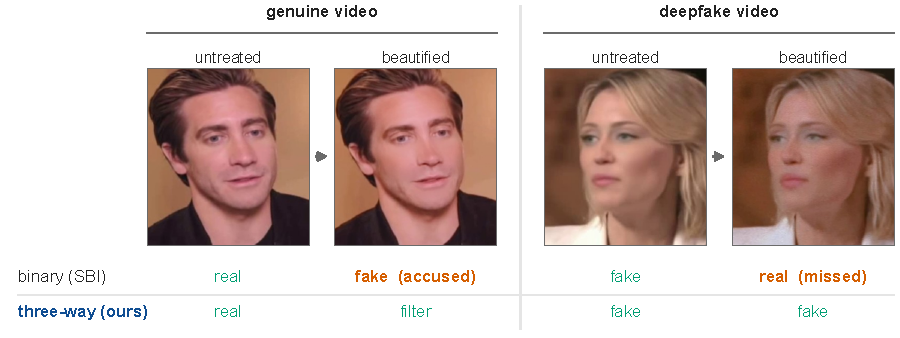
\includegraphics[width=0.84\textwidth]{fig_teaser_v5}
\captionof{figure}{Celeb-DF-B frames of a genuine video and of a deepfake, before and after the same app preset. SBI, at the
threshold that accuses 5\% of untreated genuine frames, accuses the beautified genuine face and lets the beautified deepfake
pass; our full-data three-way model calls the first \emph{filter} and the second \emph{fake} (green: correct, orange: error). The frames were selected where SBI
errs after beautification and our model is correct, so they show the two errors, not their rates. Over the benchmark SBI
accuses 1.8\% of beautified genuine frames and misses 79.8\% of beautified deepfakes; our model accuses 9.5\%, sends 47.4\%
to \emph{filter} and misses 40.7\% (Table~\ref{tab:twosided}).}\label{fig:teaser}
\end{center}\vspace{0.1\baselineskip}}
\maketitle

\begin{abstract}
Many genuine faces reaching a forgery detector were beautified by a camera app or retouching service. We measure both
errors of seventeen published detectors with one rule: the threshold on the forgery probability accuses 5\% of each source's
untreated genuine faces, and both accused genuine faces and missed forgeries are counted. Under the app
presets of Celeb-DF-B, every detector that detects the untreated forgeries loses frame AUC beyond the loss from re-encoding
alone, by 0.07--0.09 for the four CLIP-based detectors of 2025--26. On 2,210 FFHQ originals and their renders by a commercial
service, fifteen detectors score the strongest skin smoothing above its own original in 89--99\% of pairs, and thirteen accuse
36--69\% of those faces; the service's whitening, slimming and eye enlarging stay near the 5\% floor. In controlled training
on FF++ (three seeds), beautified views shown on genuine faces only raise the misses on beautified deepfakes, and skin
smoothing shown on genuine faces only makes the detector miss 96--100\% of bilaterally smoothed forgeries. A smoothing view applied to
both classes in the same form stops the accusation of commercially smoothed faces under LoRA tuning of CLIP, not under
Effort's tuning scheme. A full-data model retrained with that view misses 28--34 points more whole-crop-smoothed forgeries at
the fixed threshold, although its frame AUC with both classes smoothed is above the no-exposure baseline. Evidence maps supervised
with exact edit footprints localise held-out part-level forgeries (IoU 0.83), and restoring the named region removes about as
many detections as restoring the true footprint.
\end{abstract}

% ----------------------------------------------------------------------------
\section{Introduction}
Face-forgery detectors are used for content moderation, remote identity checks and fact-checking. In these settings a genuine
face called fake accuses a real person, and a forgery called real is let through. Many genuine faces have been beautified:
retouching is common on social media and appears even on identification documents~\cite{bharati2016,rathgeb2019}, skin
smoothing, whitening, eye enlargement and face slimming are default options in camera apps and are sold by retouching
services, and colour presets ship with every photo-sharing app. Beautification edits the pixels a forgery detector inspects
but does not change who is shown or what the person does. Biometric work has measured its effect on face
recognition~\cite{rathgeb2019} and detected retouching as such~\cite{bharati2016,jain2018}; how it moves a forgery detector in
each direction has been measured for at most six detectors at a time~\cite{libourel2024,saeed2025,concas2025}.

We score seventeen published detectors with one rule that counts both errors: Xception~\cite{xception},
EfficientNet-B4~\cite{efficientnet}, F3Net~\cite{f3net}, SPSL~\cite{spsl}, UCF~\cite{ucf}, RECCE~\cite{recce}, CORE~\cite{core},
SRM~\cite{srm}, SBI~\cite{sbi}, CADDM~\cite{caddm} and LAA-Net~\cite{laanet}, the CLIP-based Effort~\cite{effort}, Forensics
Adapter~\cite{forensicsadapter}, GenD~\cite{gend2026} and DFD-HR~\cite{dfdhr2026}, and two general generated-image detectors,
UnivFD~\cite{univfd} and NPR~\cite{npr}. They are scored on three sources of app presets and colour filters and on a commercial retouching service where each
render can be compared with its own original without a threshold. The largest failure is skin smoothing: the detectors score a
smoothed genuine face as more forged than the same face untouched, in nearly every pair. A probe of one FF++-trained CLIP model
shows a separate effect for colour filters: the two filters with a radial luminance overlay move a genuine face toward
``forged'' far more than pure colour looks do.

We then ask what training does to these errors, holding architecture, data and recipe fixed and varying only which class
receives beautified views. This is shortcut learning~\cite{geirhos2020} and class-dependent
augmentation~\cite{balestriero2022} in a setting where the sign of the resulting error can be measured. Beautified views on
genuine faces only, the direction of fine-tuning on enhanced genuine samples~\cite{saeed2025}, raise the misses on beautified
deepfakes; skin smoothing on genuine faces only teaches that smoothed means genuine, and a forger who smooths the forgery is
let through. A view whose form differs between the classes is learnt as a label in the other direction. A smoothing view
drawn in the same way for both classes removes the accusation of commercially smoothed faces for LoRA-tuned CLIP, at a stated
cost in misses on smoothed forgeries; it does not transfer to Effort's tuning scheme.

Our contributions are:
\begin{itemize}
\item \textbf{A two-sided measurement with one rule.} Seventeen detectors under app presets with re-encoding separated from
beautification on both errors, two colour-filter sources, and a commercial service read pair by pair, with per-operation
dose response and a null result on three of its four operations that controls for its rendering pipeline.
\item \textbf{Which class sees beautification.} Controlled arms over three seeds showing that beautified views on one class
move errors between misses and false alarms without changing separability, and a pre-registered chain on skin smoothing that
finds an evasion route (genuine-only smoothing), a class-asymmetric form learnt as a label, and a class-symmetric view that
avoids both under LoRA tuning, with its cost and its failure under a second tuning scheme.
\item \textbf{Reference models and a restoration test.} Full-data CLIP models trained with these views, reported with their
weaknesses (a binary control trained on the same data detects better; reenactment detection is poor), and evidence maps
evaluated by localisation and by restoring the named region.
\end{itemize}
Methods that did not help are summarised in Sec.~\ref{sec:negative}.

% ----------------------------------------------------------------------------
\section{Related Work}
\textbf{Beautification and forgery detection.} Libourel et al.~\cite{libourel2024} released Celeb-DF-B and report video AUC
drops for three detectors under app presets; Saeed et al.~\cite{saeed2025} show that face enhancement lets deepfakes evade six
detectors and fine-tune on enhanced samples; Concas et al.~\cite{concas2025} report both errors for two CNNs under a smoothing
filter. None scores detectors by a common rule or trains against the edit with a class-controlled design. On a million
smartphone photographs, von Stryk and Keuper~\cite{laionmobile2026} find that the false-alarm rate of a generated-image detector
is set by where its threshold was calibrated. Retouching detection and restoration~\cite{bharati2016,jain2018,wang2019photoshop,
retouchingffhq,frrffusion,mofrr,reface} have no forgery class; Liu et al.~\cite{miea2026} attribute forgery and beautification
tools in a closed set. Perturbation benchmarks for forgery detection~\cite{deeperforensics2020,moire2025} and for
classification~\cite{hendrycks2019} treat edits as corruptions of one class.

\textbf{Shortcuts and attacks.} Shortcut learning~\cite{geirhos2020} and group shifts~\cite{sagawa2020} describe a model that
learns a feature correlated with the label; Balestriero et al.~\cite{balestriero2022} show that augmentation and regularisation
act differently per class. StatAttack~\cite{statattack2023} and AdvShadow~\cite{advshadow2024} optimise natural appearance
changes so that forgeries pass, Fatima et al.~\cite{fatima2025} train on the worst of random counter-forensic transforms, and
semantic adversarial training exists for classification~\cite{hosseini2018,laidlaw2019,gat2023,ava2021}.

\textbf{Generalisable forgery detection.} Face X-ray~\cite{facexray} and SBI~\cite{sbi} synthesise blending artefacts,
UCF~\cite{ucf} separates common from method-specific features, LSDA~\cite{lsda} augments forgery features in latent space for
cross-method generalisation, and Effort, Forensics Adapter, GenD and DFD-HR adapt CLIP ViT-L/14. The alpha-blending
hypothesis~\cite{alphablend2026} holds that frame-based detectors read compositing artefacts, and its authors ensemble a
blending detector with blend-resistant models; our fusion of a texture-reading detector with CADDM~\cite{caddm} follows that
idea. DeepfakeBench~\cite{deepfakebench} and DF40~\cite{df40} provide checkpoints and test sets.

\textbf{Explanations.} Joint detection and segmentation of manipulated faces~\cite{nguyen2019multitask,hifinet2023} and
attention trained so that erasing it removes the evidence~\cite{gain} precede our footprint-supervised maps; amortised
maskers~\cite{dabkowski2017,phang2020} and DOLOS~\cite{dolos} localise edits, and multimodal models such as
FakeVLM~\cite{fakevlm2025} explain detections in text. Our addition is a restoration test against the true footprint.

% ----------------------------------------------------------------------------
\section{Problem and Evaluation Rule}
\label{sec:protocol}
\textbf{Classes.} A face image is \emph{forged} if it shows a person, an expression, a motion or speech that was not captured:
another identity in whole or in part, a reenactment or lip-sync, or a face or a facial feature (eye, nose, mouth) replaced by
new content. It
is \emph{beautified} if its colour, tone, skin texture or the smooth shape of the person's own features were edited after
capture while identity, expression, pose and speech stay those of the capture. The label follows what changed, not the tool: a
retouching service that smooths skin with a neural network beautifies, and a reenactment that keeps the identity forges. The
two attributes are independent, and a beautified forgery is forged. Table~\ref{tab:boundary} lists the cases near the boundary
(the supplement extends it to 17 rows, Table~\ref{S-tab:labels}). Regenerating a part of the same person by inpainting is the
case the wording does not settle: the new part was not captured, so we label it forged, but we have not measured identity or
expression preservation for any edit family, so the boundary is stated, not operationalised.

\begin{table}[t]
\centering
\caption{Cases near the class boundary. ``Scored'': whether a test set of this paper contains the case.}
\label{tab:boundary}
\footnotesize
\setlength{\tabcolsep}{2.5pt}
\begin{tabular}{@{}>{\raggedright\arraybackslash}p{0.47\columnwidth}>{\raggedright\arraybackslash}p{0.2\columnwidth}>{\raggedright\arraybackslash}p{0.27\columnwidth}@{}}
\toprule
Case & Label & Scored \\
\midrule
Colour preset, skin smoothing, whitening, slimming, eye enlargement (app or service, neural or not) & beautified & presets, filters, one service \\
Face swap; reenactment & forged & FF++, Celeb-DF, DFD, DF40 \\
A part from another person & forged & part-level set \\
A part of the same person regenerated by inpainting & forged (boundary) & part-level set \\
Beautified forgery & forged & Celeb-DF-B, smoothed forgeries \\
Entire-face synthesis, attribute editing, lip-sync & forged & not scored \\
\bottomrule
\end{tabular}
\end{table}

\textbf{Requirement and rule.} A detector should return a forgery score that does not move when a face is beautified; whether a
face was beautified may be reported to the user as a separate attribute (evaluated in Sec.~\ref{S-sec:native}), and every
detection number reads the forgery score only. Each detector is
scored by its probability of forgery $P(\text{fake})$. On every source the threshold is the one that accuses 5\% of that
source's untreated genuine frames. It is fitted per source, which no deployed detector can do; it gives every detector an operating
point fitted to its own untreated data, and on the retouching service we also report statistics that need no threshold. Under
beautification we report the false-alarm rate FA (genuine faces called fake) and the miss rate MISS (forgeries not called
fake). A forgery that a three-way model sends to its beautified class is a miss. Every AUC is labelled frame or video level;
video scores are means of frame scores. Intervals are 95\% percentile bootstraps that resample videos (Celeb-DF-B, the filter
sources, DF40) or originals (the service), with the threshold re-estimated in every draw: 1,000 draws for Celeb-DF-B, DF40,
the smoothed-forgery test and the service, 500 for the filter sources. Videos of one person are not resampled together, so the
intervals on Celeb-DF and DFD are narrower than identity-level intervals would be. Differences between models use identical
draws. We do not correct for multiple comparisons except where stated.

\textbf{Sources.} \emph{Celeb-DF-B}~\cite{libourel2024}: 232 Celeb-DF-v2 videos per condition (as recorded, re-encoded,
beautified by one of four app presets; genuine and synthesised), 32 frames each; 231 have a detected face in the untreated
and 230 in the beautified genuine condition. The treated videos are re-framed to portrait with tinted bars, and our face
detector missed 57\% of their faces; after reading that result we trimmed uniform bars from all six conditions before
detection. This fix is post hoc, and face size and resampling still differ between untreated and treated frames, which the
re-encoded control does not reproduce. We report re-encoding alone and its difference from the preset on both errors:
$\Delta$MISS$_\text{beauty}$ and $\Delta$FA$_\text{beauty}$ are the rise under the preset minus the rise under re-encoding,
and AUC$_c{-}$AUC$_b$ is the AUC lost beyond re-encoding. \emph{Celeb-DF-v2 filters}: 516 test videos~\cite{celebdf}, each
frame also under one of eleven colour filters~\cite{pilgram} never used in training; this set was used to diagnose the filter
effect and is a development source. \emph{DFD filters}: 332 DFD videos~\cite{dfd} under one of sixteen filters from a second
library, built after every method decision. \emph{Commercial retouching}: 2,210 FFHQ originals and their renders by Alibaba
from RetouchingFFHQ~\cite{retouchingffhq} (four operations, three levels). No model was trained on this service, but more than
60 of our checkpoints and all 17 published detectors have been scored on it, the strongest smoothing level (Smoothing-90) was
singled out after reading it, and the pre-declared bars of Sec.~\ref{sec:chain} are defined on it; it is an analysis set, not
a clean test. Its originals share no image with the 7,831 FFHQ training originals (a disjoint index range; FFHQ has no
identity labels). \emph{Untreated detection}: Celeb-DF-v2, DFD and the held-out methods of DF40~\cite{df40}.

\begin{table}[t]
\centering
\caption{Models and arms. All use CLIP ViT-L/14 with rank-16 LoRA (or Effort's SVD-residual tuning where noted) and the
training pipeline of Sec.~\ref{sec:method}. ``Views'': which class receives beautified training views.}
\label{tab:notation}
\footnotesize
\setlength{\tabcolsep}{2.5pt}
\begin{tabular}{@{}>{\raggedright\arraybackslash}p{0.27\columnwidth}>{\raggedright\arraybackslash}p{0.56\columnwidth}c@{}}
\toprule
Name & Data, views, head & seeds \\
\midrule
P0, P1, P2 & FF++ only, forged head; views on no class, genuine only, both & 3 \\
P1-smooth & P1 with smoothing as the only view & 3 \\
P2-smooth, P2-nosmooth & P2 with smoothing only, with smoothing removed & 2 \\
P2-sym & smoothing as the only view, same form on both classes & 2 \\
Effort scheme & P0 and P2 (2 seeds), P2-sym (1 seed), SVD-residual tuning & 1--2 \\
\ours{} & full data$^\dagger$, P2 views, three-way head & 2 \\
\ours{} variant & \ours{} with the class-symmetric smoothing view & 1 \\
binary control & \ours{} data and views, forged head only & 1 \\
\bottomrule
\multicolumn{3}{@{}p{0.97\columnwidth}@{}}{\scriptsize $^\dagger$FF++ plus 7,831 FFHQ originals, their renders by two retouching services (Tencent, Megvii) and the single-operation components of those renders, and 61,510 part-level forgeries. The published CLIP detectors were trained on FF++ alone.}\\
\end{tabular}
\end{table}

% ----------------------------------------------------------------------------
\section{Method}
\label{sec:method}
Every edited training image has a pixel-aligned original $x_0$, so the footprint of the edit is exact,
$M(x)=\mathrm{dilate}_\rho(\mathbf{1}[\|x-x_0\|_\infty>\tau])$ with $\tau=6$ on 8-bit intensities.

\textbf{FF++ triplets.} FF++ c23~\cite{ffpp}, official 720/140/140 video split. For each genuine training frame $x_0$ a step
draws a genuine item, a beautified item (one of four landmark and skin operations at a random strength, one of 14 colour
filters~\cite{pilgram}, or a random colour grading) and a forged item (a self-blend of $x_0$~\cite{sbi}, an observed FF++
forgery, or a part-level forgery), and the forged item is beautified with probability 0.5. Forged items without landmarks
receive skin smoothing as a whole-crop filter, not as the face-local operation; Sec.~\ref{sec:chain} shows what this asymmetry
teaches. The same random blur or downscale is applied to all three items. The FF++-only arms use nothing else.

\textbf{Commercial renders and part-level forgeries.} The full-data models add 7,831 FFHQ photographs~\cite{ffhq} and their
renders by Tencent and Megvii~\cite{retouchingffhq}, sister services of the test service with the same four operations. Each
render is split by dense optical flow~\cite{dis} and a photometric residual into eye and contour warps and low- and
high-frequency photometric components in the original's geometry (supplement, Alg.~\ref{S-alg:decomp}); 50,112 of 73,952
components lie above the noise floor. A render's photometric residual is also added to a self-blend of the same original.
61,510 part-level forgeries on FF++ frames transplant the eyes, nose or mouth of another identity or regenerate the part with
Stable Diffusion inpainting, with pixels outside the feathered mask copied from $x_0$; the held-out set uses test frames and
test donors.

\textbf{Model.} A frozen CLIP ViT-L/14~\cite{clip} with rank-16 LoRA~\cite{lora} on every attention projection (3.2\,M of
306\,M parameters trained). Two linear heads on the pooled feature give the forged logit $z_f$ and the beautified logit $z_b$;
$P(\text{fake})=\sigma(z_f)$ and $P(\text{filter})=(1-\sigma_f)\sigma_b$, so the forgery score does not depend on $z_b$. An
operation-presence head and a $1\times1$ convolution on the spatial tokens (the evidence map $\hat m$, $16\times16$) are
trained against the operation labels and $M$ with BCE and Dice; the classifier does not read $\hat m$. Training: 224\,px,
AdamW at $10^{-4}$, 8 epochs, 16 genuine bases per batch. Checkpoints are chosen on validation data only (FF++ validation
macro-F1; for full-data models its mean with balanced accuracy on held-out originals and renders of the training services).

% ----------------------------------------------------------------------------
\section{Results}
\label{sec:results}
\begin{table*}[t]
\centering
\caption{Both errors under one rule ($P(\text{fake})$, threshold at 5\% FPR on each source's untreated genuine frames).
Celeb-DF-B: AUC untreated, re-encoded (AUC$_c$) and beautified (AUC$_b$), AUC lost beyond re-encoding, rise in misses and in
false alarms under the preset minus the rise under re-encoding, and FA$_b$, the false-alarm rate on beautified genuine frames.
DFD: sixteen held-out filters on the full frame. Percentage points. Intervals, the Celeb-DF-v2 filter source and video-level
AUC in the supplement (Tables~\ref{S-tab:twosidedfull} and~\ref{S-tab:cdfbextra}). $^\ddagger$General generated-image detectors,
not trained on faces. $^\dagger$Trained on more data than the published detectors (Table~\ref{tab:notation}).}
\label{tab:twosided}
\scriptsize
\setlength{\tabcolsep}{3pt}
\begin{adjustbox}{max width=\textwidth}\begin{tabular}{@{}ll ccccccc cccc@{}}
\toprule
 & & \multicolumn{7}{c}{Celeb-DF-B, app presets (frame level)} & \multicolumn{4}{c}{DFD + 16 held-out filters (frame level)} \\
\cmidrule(lr){3-9}\cmidrule(lr){10-13}
Detector & train & AUC & AUC$_c$ & AUC$_b$ & AUC$_c{-}$AUC$_b$ & $\Delta$MISS$_\text{beauty}$ & FA$_b$ & $\Delta$FA$_\text{beauty}$ & AUC & AUC$_f$ & $\Delta$MISS & $\Delta$FA \\
\midrule
Xception~\cite{xception} & FF++ c23 & 0.811 & 0.795 & 0.737 & 0.058 & +10.9 & 5.7 & -1.7 & 0.854 & 0.834 & +2.0 & +2.0 \\
EfficientNet-B4~\cite{efficientnet} & FF++ c23 & 0.811 & 0.798 & 0.762 & 0.035 & +3.4 & 7.8 & +1.7 & 0.810 & 0.781 & +6.3 & -0.5 \\
F3Net~\cite{f3net} & FF++ c23 & 0.798 & 0.782 & 0.731 & 0.051 & +10.9 & 5.4 & -1.9 & 0.781 & 0.774 & -8.5 & +3.6 \\
SPSL~\cite{spsl} & FF++ c23 & 0.781 & 0.769 & 0.727 & 0.042 & +12.4 & 3.4 & -2.4 & 0.829 & 0.837 & +4.7 & -1.8 \\
UCF~\cite{ucf} & FF++ c23 & 0.841 & 0.829 & 0.777 & 0.053 & +11.3 & 5.7 & +0.2 & 0.822 & 0.804 & +5.0 & +0.3 \\
RECCE~\cite{recce} & FF++ c23 & 0.785 & 0.765 & 0.723 & 0.042 & +13.8 & 4.1 & -3.6 & 0.833 & 0.808 & +7.3 & -0.2 \\
CORE~\cite{core} & FF++ c23 & 0.821 & 0.808 & 0.752 & 0.057 & +13.5 & 4.0 & -2.2 & 0.827 & 0.821 & -5.4 & +1.6 \\
SRM~\cite{srm} & FF++ c23 & 0.789 & 0.769 & 0.733 & 0.035 & +15.3 & 2.8 & -3.4 & 0.830 & 0.822 & +5.8 & +0.2 \\
SBI~\cite{sbi} & FF++ c23 & 0.875 & 0.861 & 0.752 & 0.109 & +21.8 & 1.8 & -0.6 & 0.829 & 0.810 & +4.5 & +0.4 \\
UnivFD$^\ddagger$~\cite{univfd} & ProGAN$^\ddagger$ & 0.653 & 0.637 & 0.624 & 0.013 & -7.2 & 7.6 & +4.5 & 0.840 & 0.801 & -10.2 & +11.6 \\
NPR$^\ddagger$~\cite{npr} & ProGAN$^\ddagger$ & 0.503 & 0.503 & 0.498 & 0.006 & -0.7 & 3.4 & +0.9 & 0.473 & 0.516 & -13.7 & +9.4 \\
Effort~\cite{effort} & FF++ c23 & 0.909 & 0.882 & 0.807 & 0.075 & +11.0 & 5.4 & +2.1 & 0.939 & 0.905 & +15.1 & -2.3 \\
Forensics Adapter~\cite{forensicsadapter} & FF++ c23 & 0.909 & 0.894 & 0.828 & 0.066 & +15.2 & 7.9 & +0.1 & 0.940 & 0.924 & +8.0 & -0.6 \\
GenD~\cite{gend2026} & FF++ c23 & 0.924 & 0.898 & 0.807 & 0.091 & +12.0 & 9.9 & +3.6 & 0.934 & 0.925 & +3.1 & +1.2 \\
DFD-HR~\cite{dfdhr2026} & FF++ c23 & 0.938 & 0.915 & 0.838 & 0.077 & +3.6 & 14.6 & +9.8 & 0.943 & 0.928 & +9.1 & -2.0 \\
CADDM~\cite{caddm} & FF++ raw & 0.886 & 0.850 & 0.762 & 0.088 & -2.9 & 13.8 & +9.9 & 0.845 & 0.818 & +3.8 & +0.8 \\
LAA-Net~\cite{laanet} & FF++ raw & 0.889 & 0.870 & 0.698 & 0.172 & +14.7 & 6.0 & +3.3 & 0.810 & 0.783 & +6.2 & +0.0 \\
\midrule
P0 & FF++ & 0.927 & 0.901 & 0.860 & 0.041 & +17.0 & 5.1 & -1.6 & 0.943 & 0.924 & +9.3 & -0.2 \\
P2-sym & FF++ & 0.920 & 0.900 & 0.866 & 0.034 & +14.2 & 5.5 & -1.2 & 0.936 & 0.921 & +7.3 & -0.4 \\
\ours{}$^\dagger$ & FF++, FFHQ & 0.938 & 0.918 & 0.866 & 0.052 & +6.7 & 9.5 & +4.9 & 0.942 & 0.931 & +8.9 & -1.0 \\
\quad second seed$^\dagger$ & FF++, FFHQ & 0.941 & 0.926 & 0.883 & 0.043 & +8.3 & 6.7 & +2.7 & 0.945 & 0.931 & +4.4 & +0.3 \\
\quad \ours{} variant$^\dagger$ & FF++, FFHQ & 0.941 & 0.925 & 0.868 & 0.057 & +10.0 & 9.2 & +4.9 & 0.947 & 0.934 & +8.5 & -0.9 \\
binary control$^\dagger$ & FF++, FFHQ & 0.949 & 0.934 & 0.896 & 0.038 & +7.0 & 7.4 & +2.3 & 0.961 & 0.952 & +4.2 & +0.2 \\
\bottomrule
\end{tabular}
\end{adjustbox}
\end{table*}

\begin{table}[t]
\centering
\caption{Commercial skin smoothing (Smoothing-90): 2,210 FFHQ originals and their renders. Share of renders scored above their
own original (50 means no shift), medians of $P(\text{fake})$, median paired shift of the forgery logit with a bootstrap
interval over originals, and share of renders above the threshold that accuses 5\% of the originals. NPR scores everything at
1.0. All renders and operations in the supplement.}
\label{tab:retouch}
\scriptsize
\setlength{\tabcolsep}{2.5pt}
\begin{adjustbox}{max width=\columnwidth}\begin{tabular}{@{}l cccc@{}}
\toprule
Detector & above own orig.\ (\%) & median $P(\text{fake})$ & median $\Delta$logit [95\% CI] & accused (\%) \\
\midrule
Xception~\cite{xception} & 95.2 & 0.29 $\rightarrow$ 0.94 & +3.32 [+3.17, +3.45] & 51.6 \\
EfficientNet-B4~\cite{efficientnet} & 93.7 & 0.32 $\rightarrow$ 0.96 & +3.48 [+3.33, +3.57] & 36.3 \\
F3Net~\cite{f3net} & 97.8 & 0.13 $\rightarrow$ 0.97 & +4.92 [+4.74, +5.08] & 50.6 \\
SPSL~\cite{spsl} & 97.3 & 0.46 $\rightarrow$ 0.96 & +3.05 [+2.95, +3.12] & 51.2 \\
UCF~\cite{ucf} & 95.4 & 0.03 $\rightarrow$ 0.98 & +5.47 [+5.20, +5.73] & 41.4 \\
RECCE~\cite{recce} & 96.5 & 0.12 $\rightarrow$ 0.94 & +3.82 [+3.70, +3.96] & 36.8 \\
CORE~\cite{core} & 96.6 & 0.25 $\rightarrow$ 0.95 & +3.90 [+3.74, +4.03] & 54.8 \\
SRM~\cite{srm} & 99.3 & 0.46 $\rightarrow$ 0.67 & +0.68 [+0.65, +0.71] & 62.8 \\
SBI~\cite{sbi} & 96.2 & 0.21 $\rightarrow$ 0.99 & +4.88 [+4.72, +5.04] & 37.3 \\
UnivFD$^\ddagger$~\cite{univfd} & 90.4 & 0.01 $\rightarrow$ 0.02 & +1.22 [+1.17, +1.28] & 16.6 \\
NPR$^\ddagger$~\cite{npr} & n/a & n/a & n/a & n/a \\
Effort~\cite{effort} & 95.6 & 0.32 $\rightarrow$ 0.59 & +0.96 [+0.90, +1.02] & 43.2 \\
Forensics Adapter~\cite{forensicsadapter} & 93.3 & 0.06 $\rightarrow$ 0.35 & +1.72 [+1.59, +1.87] & 39.7 \\
GenD~\cite{gend2026} & 98.5 & 0.23 $\rightarrow$ 0.92 & +3.27 [+3.19, +3.35] & 68.7 \\
DFD-HR~\cite{dfdhr2026} & 99.0 & 0.21 $\rightarrow$ 0.71 & +2.06 [+1.93, +2.15] & 64.9 \\
CADDM~\cite{caddm} & 60.9 & 0.54 $\rightarrow$ 0.74 & +0.67 [+0.53, +0.81] & 6.3 \\
LAA-Net~\cite{laanet} & 89.2 & 0.23 $\rightarrow$ 0.97 & +3.60 [+3.36, +3.79] & 17.2 \\
\midrule
P0 & 98.5 & 0.05 $\rightarrow$ 0.97 & +5.17 [+5.05, +5.38] & 54.2 \\
P2-sym & 53.7 & 0.02 $\rightarrow$ 0.02 & +0.09 [+0.03, +0.12] & 5.9 \\
\ours{}$^\dagger$ & 32.5 & 0.00 $\rightarrow$ 0.00 & -1.20 [-1.28, -1.12] & 8.6 \\
\quad \ours{} variant$^\dagger$ & 30.0 & 0.00 $\rightarrow$ 0.00 & -1.09 [-1.19, -1.00] & 8.1 \\
binary control$^\dagger$ & 70.5 & 0.00 $\rightarrow$ 0.00 & +0.41 [+0.38, +0.44] & 9.1 \\
\bottomrule
\end{tabular}
\end{adjustbox}
\end{table}

\subsection{Both errors under one rule}
\label{sec:measure}
\textbf{Commercial retouching.} Table~\ref{tab:retouch} reads the Smoothing-90 renders against their own originals. Fifteen of
the seventeen detectors score the render above its original in 89--99\% of pairs, and the median $P(\text{fake})$ moves from
0.21 to 0.99 for SBI and from 0.23 to 0.92 for GenD: a heavily smoothed genuine face is scored like a forgery whatever the
threshold. The exceptions are NPR, saturated, and CADDM (60.9\%). At the threshold that accuses 5\% of the originals thirteen
detectors accuse 36.3--68.7\% of the renders; UnivFD, LAA-Net and CADDM accuse 16.6, 17.2 and 6.3\%, but eight detectors have a
threshold above 0.96 on these stills, so the threshold-free columns are the ones to read first. Whitening, face slimming and eye
enlarging at their strongest level stay at 3.7--8.1\% for thirteen of the sixteen detectors other than NPR (Effort 16.8\% on
eye enlarging, UnivFD 11.7\%, DFD-HR 9.6\%), and smoothing is dose-dependent across levels 30, 60 and 90 for every detector
except CADDM (Table~\ref{S-tab:v4perop}). The three operations go through the same service, encoder and resolution as the
smoothing, so the accusation is not an artefact of the rendering pipeline: the retouching result is a smoothing result.
A sign test rejects ``no shift'' for every published detector other than NPR ($p<10^{-10}$), and the median paired shift of
the forgery logit is $+0.7$ to $+5.5$. Our full-data three-way models move the other way: \ours{} scores the render \emph{below} its
original in 67.5\% of pairs (median logit shift $-1.20$ [$-1.28$, $-1.12$]; second seed $-0.53$), so smoothing moves its score
toward genuine. Only the FF++-only symmetric arm P2-sym stays close to no shift ($+0.09$ [$+0.03$, $+0.12$] and $+0.03$
[$0.00$, $+0.09$]). Our full-data models were trained on renders of the two sister services (marked $^\dagger$), which the
published detectors were not.

\textbf{App presets.} On Celeb-DF-B every detector that detects the untreated forgeries loses frame AUC beyond what
re-encoding costs (Table~\ref{tab:twosided}): SBI 0.861 to 0.752 against the re-encoded frames, CADDM 0.850 to 0.762, LAA-Net
0.870 to 0.698, and 0.066--0.091 for the four CLIP detectors (Effort 0.075, Forensics Adapter 0.066, GenD 0.091, DFD-HR
0.077). At video level CADDM goes from 0.965 to 0.832 (0.933 re-encoded), against 0.91 to 0.76 reported by Libourel et al.~\cite{libourel2024}. The
errors fall on different sides. Beyond re-encoding, the presets raise the miss rate by 21.8 (SBI), 11.0 (Effort), 15.2
(Forensics Adapter), 12.0 (GenD) and 14.7 points (LAA-Net), and raise false alarms by 9.8 (DFD-HR), 9.9 (CADDM) and 3.6 points
(GenD). CADDM's misses do not rise ($-2.9$) because the presets raise its scores for genuine frames too: it accuses 13.8\% of
beautified genuine frames. Under the DFD filters Effort's miss rate rises by 15.1 points and Forensics Adapter's by 8.0.

\subsection{Colour filters: a probe of one model}
\label{sec:mechanism}
We probed the pooled feature of one model of ours: the FF++-only three-way CLIP model (``\ours{}, FF++ only'' in
Table~\ref{S-tab:twosidedfull}), whose forgery decision is a linear head $w$ and which was trained with random colour grading and
14 colour filters as beautified views. Of the eleven held-out Celeb-DF-v2 filters, the two with a
radial luminance overlay, \emph{earlybird} and \emph{mayfair}, move the forgery logit of a genuine validation frame by $+7.8$
and $+5.6$, and the nine pure colour looks by $+0.1$ to $+2.4$; forged frames move by $-0.7$ to $+1.8$. A luminance ramp around
the face reads as forgery evidence for this model, in line with the alpha-blending hypothesis~\cite{alphablend2026}. Projecting
out the subspace spanned by training-time beautification shifts and refitting the head does not help: against a refit without
erasure (clean AUC 0.985, false alarms under filters 15.8\%), erasing 2--32 directions lowers the clean AUC to 0.919--0.933 and
raises the false alarms to 18.3--19.2\% (Table~\ref{S-tab:erasure}). This probe covers two filters and one model of ours; it
does not explain the smoothing result, and the direction does not hold for every published detector (Effort's false alarms
fall under the Celeb-DF-v2 filters while its misses rise by 23.3 points).

\subsection{Which class receives beautified views}
\label{sec:exposure}
With architecture, data and recipe fixed, P0, P1 and P2 differ only in which class receives beautified views
(Table~\ref{tab:notation}). On Celeb-DF-B the beautification-specific miss rise is 17.0, 14.2 and 10.8 points for P0 (three
seeds), 21.5, 21.8 and 20.4 for P1 and 9.8, 10.3 and 12.8 for P2 (Table~\ref{S-tab:exposure}). P1 exceeds P0 by 4.5--9.5 points
in every seed and P2 by 7.5--11.7; all three P1$-$P0 contrasts remain significant after a Holm correction over the nine exposure contrasts of the three seeds (adjusted $p\le0.01$; Sec.~\ref{S-sec:exposure}). Beautification shown on genuine faces only is learnt as a sign of a genuine face. P2
against P0 is $-7.2$, $-4.0$ and $+2.0$ points: significant in each seed, but of changing sign and within the seed spread of P0
itself. On the two filter sources P2 lowers the miss
rise by 5--10 points in 9 of 10 seed-by-source cells and raises the false-alarm rise by 2--5 points, while the frame AUC under
the filters does not change. Exposure moves errors between misses and false alarms; it does not make the classes more
separable. Under Effort's tuning scheme, P2 also lowers the miss rise against P0 ($-4.6$ and $-5.2$ points, two seeds); P1 was
not trained under that scheme. The fourth cell, views on forged faces only, was not trained. The no-exposure CLIP model already
keeps more frame AUC under the presets (0.860--0.883) than Effort's released checkpoint (0.807), so most of the margin of our
models over the CLIP baselines comes from the base recipe, not from exposure.

\begin{table*}[t]
\centering
\caption{What each training recipe buys and costs, per seed (1 / 2 / 3 where trained; ``--'' not scored); names as in
Table~\ref{tab:notation}. Commercial Smoothing-90 as in Table~\ref{tab:retouch}. Smoothed Celeb-DF-v2: change of the miss rate on
forgeries under the strong whole-crop bilateral filter at the threshold of 5\% FPR on untreated genuine frames (a negative value
comes from accusing every smoothed frame, genuine ones included), and frame AUC with both classes smoothed. Untreated Celeb-DF-v2
video AUC; Celeb-DF-B frame AUC under the presets; DF40 reenactment (FR) in the FF++ domain, video AUC, mean over twelve methods.
DFD, $\Delta$MISS$_\text{beauty}$, the Celeb-DF domain, every smoothing form and intervals in
Tables~\ref{S-tab:tradeofffull}, \ref{S-tab:v4evasion} and~\ref{S-tab:v4df40full}.}
\label{tab:tradeoff}
\scriptsize
\setlength{\tabcolsep}{2.5pt}
\begin{adjustbox}{max width=\textwidth}\begin{tabular}{@{}l cc cc c c c@{}}
\toprule
 & \multicolumn{2}{c}{commercial Smoothing-90} & \multicolumn{2}{c}{smoothed Celeb-DF-v2} & Celeb-DF-v2 & Celeb-DF-B & DF40 FR \\
\cmidrule(lr){2-3}\cmidrule(lr){4-5}
Arm & accused (\%) & above own orig.\ (\%) & miss rise & frame AUC & video AUC & frame AUC$_b$ & video AUC \\
\midrule
P0 & 54.2 / 56.1 / 43.5 & 98.5 / 99.0 / 97.0 & -16.0 / -11.8 / +4.3 & 0.747 / 0.736 / 0.736 & 0.938 / 0.938 / 0.940 & 0.860 / 0.883 / 0.883 & 0.906 / 0.877 / 0.873 \\
P2 & 11.7 / 7.1 / 6.9 & 84.1 / 72.4 / 75.5 & -26.5 / -13.3 / -- & 0.740 / 0.746 / -- & 0.917 / 0.920 / 0.935 & 0.879 / 0.893 / 0.877 & 0.809 / 0.785 / -- \\
P2-nosmooth & 55.3 / 67.1 & 98.6 / 99.4 & -28.9 / -33.1 & 0.732 / 0.695 & 0.913 / 0.924 & 0.879 / 0.873 & 0.858 / -- \\
P2-smooth & 2.3 / 5.3 & 27.3 / 51.7 & -48.2 / -44.6 & 0.785 / 0.734 & 0.904 / 0.926 & 0.865 / 0.870 & 0.779 / 0.833 \\
P1 & 3.7 / 7.1 / 4.6 & 43.5 / 67.5 / 64.3 & +51.2 / -- / -- & 0.587 / -- / -- & 0.900 / 0.910 / 0.923 & 0.844 / 0.851 / 0.864 & 0.807 / -- / -- \\
P1-smooth & 0.7 / 1.0 / 0.9 & 2.6 / 6.5 / 5.4 & +56.4 / +60.0 / +62.9 & 0.643 / 0.579 / 0.596 & 0.922 / 0.929 / 0.939 & 0.887 / 0.896 / 0.893 & 0.871 / 0.869 / 0.900 \\
P2-sym & 5.9 / 6.1 & 53.7 / 51.8 & +14.6 / +17.5 & 0.767 / 0.796 & 0.919 / 0.934 & 0.866 / 0.888 & 0.871 / 0.796 \\
Effort scheme, P0 & 56.9 / 63.2 & 99.1 / 99.1 & -32.2 / -- & 0.719 / -- & 0.944 / 0.954 & 0.882 / 0.886 & -- / -- \\
Effort scheme, P2-sym & 14.5 & 88.4 & +24.9 & 0.757 & 0.935 & 0.890 & 0.822 \\
released Effort fine-tuned, no views & 55.3 & 98.5 & -39.9 & 0.754 & 0.926 & 0.805 & -- \\
released Effort fine-tuned, P2-sym view & 39.9 & 96.6 & -19.0 & 0.740 & 0.921 & 0.791 & 0.805 \\
\ours{} & 8.6 / 12.5 & 32.5 / 41.3 & -44.3 / -- & 0.688 / -- & 0.947 / 0.946 & 0.866 / 0.883 & 0.718 / 0.780 \\
\ours{} variant & 8.1 & 30.0 & +34.1 & 0.796 & 0.954 & 0.868 & 0.738 \\
binary control & 9.1 & 70.5 & -15.0 & 0.754 & 0.956 & 0.896 & 0.842 \\
\bottomrule
\end{tabular}
\end{adjustbox}
\end{table*}

\subsection{Skin smoothing: a chain of pre-registered arms}
\label{sec:chain}
We traced the smoothing result through FF++-only arms, each with bars written before training
(Table~\ref{tab:tradeoff}; bars and per-seed values in Sec.~\ref{S-sec:chain}). No image of any retouching service is used.
The scripted smoothing is a bilateral filter blended inside the face hull, the same kind of edit as the service's, at a strength
range set to cover the two sister services while the test service's measurements were on disk; what is tested is robustness
across implementations and image domains of one operation at matched strength. The first analysis on the service (P0, P1, P2)
was post hoc.

\textbf{No exposure reproduces the published detectors.} P0 accuses 54.2, 56.1 and 43.5\% of the Smoothing-90 renders and
scores them above their original in 97--99\% of pairs, although it trains with label-symmetric blur, rescaling and JPEG.
General beautified views lower the rate to 3.7--7.1\% (P1) and 6.9--11.7\% (P2), but P2 still ranks the render above its
original in 72--84\% of pairs.

\textbf{No other view substitutes for smoothing.} P2-nosmooth accuses 55.3\% [51.9, 58.6] and 67.1\% (two seeds). P2-smooth
lowers the accusation to 2.3 and 5.3\%, but this arm carries the form shortcut described below (it calls 47.8--88.3\% of
whole-crop-smoothed genuine frames forged), so it does not show that smoothing views alone remove the accusation for the right
reason.

\textbf{The genuine-only recipe is an evasion route.} P1-smooth accuses 0.7--1.0\% (three seeds) and ranks the render above
its original in 2.6--6.5\% of pairs. A check written before any smoothed forgery was scored applies a whole-crop bilateral
filter at three strengths and two forms no arm has seen, a $5\times5$ median filter and a 50\% blend with a Gaussian blur, to
Celeb-DF-v2 test frames. P1-smooth then misses 96--100\% of bilaterally smoothed forgeries (miss rise of 56--63 points),
75--84\% of median-filtered forgeries and 51--54\% of blended ones, against 37--44\% untreated. It has learnt that
smoothed means genuine, and its low accusation rates are this shortcut.

\textbf{A class-asymmetric form is learnt as a label.} A whole-crop bilateral filter on a \emph{genuine} frame is called forged
by \ours{} in 34.9, 79.8 and 90.1\% of frames at the three strengths and by P2-smooth in 47.8--88.3\%, against 0.8, 16.8 and
39.6\% for P0. In training, genuine items receive the face-local smoothing and forged items without landmarks the whole-crop
filter, so the form of the smoothing predicts the class.

\textbf{A class-symmetric view.} P2-sym draws both forms on both classes. Pre-declared bars: (a) Smoothing-90 accused at most
15\% with the render above its original in 25--75\% of pairs; (b) false alarms on smoothed genuine frames at most 15\% for every
form; (c) a miss rise on smoothed forgeries at most 5 points above P0's for every form; two seeds. Bars (a) and (b) are met on
both seeds: 5.9 and 6.1\%, 53.7 and 51.8\% of pairs, false alarms of 2.2--6.1\%. This is the arm whose low accusation cannot come
from the form cue. Bar (c) is not met: the miss rises are $+7.6$ to $+20.6$ and exceed P0's by more than 5 points at the mid and
strong strengths, partly because P0's miss rate falls under strong smoothing ($-16.0$ and $-11.8$) as it accuses everything
smoothed. The arm does not pass smoothed forgeries wholesale, as P1-smooth does, but its misses rise by 8--21 points at the fixed
threshold; its frame AUC with both classes smoothed (0.767 and 0.796 at the strong strength) is at or above P0's (0.736--0.747).
Its untreated Celeb-DF-v2 video AUC is 0.919 and 0.934 against 0.938. Under Effort's tuning scheme the same view meets bar (b)
but not (a): Smoothing-90 falls from 56.9 to 14.5\%, but the render is still ranked above its original in 88.4\% of pairs. The
recipe holds for LoRA tuning of CLIP, within the views we tried, and not across tuning schemes.

\textbf{The full-data model with the symmetric view.} Retrained with the symmetric view (one seed), the variant calls 1.0--1.7\%
of whole-crop-smoothed genuine frames forged (\ours{}: 34.9--90.1\%) and keeps untreated video AUC (Celeb-DF-v2 0.954, DFD
0.983 against 0.947 and 0.978). Its miss rate on whole-crop-smoothed forgeries rises by 28.1, 33.8 and 34.1 points at the three
strengths, from 43.5\% to 77.6\% at the strongest, while its frame AUC with both classes smoothed is 0.796 against 0.688 for
\ours{} and 0.754 for the binary control: smoothing shifts its scores for both classes toward genuine, and the threshold fixed on
untreated frames turns that shift into misses. The variant replaces \ours{} under its pre-declared rule only if its explanation
flip rate falls by at most 1.0 point; it fell by 1.4--1.6, the ceiling fell by the same amount and the flip rate relative to the
ceiling is unchanged ($-0.1$ to $+0.1$), so a ceiling-relative bar would have passed. We kept the bar as written; both models are
reported side by side, and with one seed of the variant neither should be read as the better detector.

\subsection{Untreated detection and DF40}
\label{sec:detect}
\begin{table}[t]
\centering
\caption{DF40 held-out, untreated: video AUC, mean over nine face-swap (FS) and twelve reenactment (FR) methods, against the
same-domain real videos. All detectors share one crop. Intervals and paired differences in Table~\ref{S-tab:v4df40full}.}
\label{tab:df40}
\footnotesize
\setlength{\tabcolsep}{3pt}
\begin{adjustbox}{max width=\columnwidth}\begin{tabular}{@{}l cc cc@{}}
\toprule
 & \multicolumn{2}{c}{FF++ domain} & \multicolumn{2}{c}{Celeb-DF domain} \\
\cmidrule(lr){2-3}\cmidrule(lr){4-5}
Detector & FS & FR & FS & FR \\
\midrule
eight CNNs (range) & 0.766--0.860 & 0.754--0.859 & 0.656--0.736 & 0.671--0.740 \\
Effort~\cite{effort} & 0.944 & 0.808 & 0.935 & 0.710 \\
Forensics Adapter~\cite{forensicsadapter} & 0.948 & 0.828 & 0.897 & 0.665 \\
GenD~\cite{gend2026} & 0.966 & 0.935 & 0.947 & 0.828 \\
DFD-HR~\cite{dfdhr2026} & 0.982 & 0.932 & 0.940 & 0.698 \\
CADDM~\cite{caddm} & 0.869 & 0.794 & 0.788 & 0.541 \\
\midrule
\ours{} & 0.952 & 0.718 & 0.905 & 0.502 \\
\quad second seed & 0.960 & 0.780 & 0.928 & 0.559 \\
\quad \ours{} variant & 0.952 & 0.738 & 0.909 & 0.539 \\
binary control & 0.969 & 0.842 & 0.926 & 0.647 \\
P0 & 0.981 & 0.906 & 0.925 & 0.692 \\
P2-sym & 0.968 & 0.871 & 0.913 & 0.670 \\
\bottomrule
\end{tabular}
\end{adjustbox}
\end{table}
\textbf{Celeb-DF-v2 and DFD.} Each DeepfakeBench-trained baseline is scored on its own crop and \ours{} on ours, with paired
intervals over common videos (Table~\ref{S-tab:reproduce}). \ours{} (frame AUC 0.891 on Celeb-DF-v2, 0.942 on DFD) is on par
with Effort and Forensics Adapter (paired frame-AUC differences $[-0.013, 0.038]$ and $[-0.030, 0.013]$; $[-0.006, 0.025]$ and
$[-0.013, 0.017]$); our Effort reproduction is below its published Celeb-DF-v2 video AUC (0.927 against 0.956). The binary
control trained on the same data is better (frame AUC 0.914 and 0.961). Under the presets \ours{} keeps a frame AUC$_b$ of 0.866 and 0.883
(two seeds); the paired differences against Effort, Forensics Adapter, GenD and DFD-HR are $+0.059$, $+0.038$, $+0.059$ and $+0.028$ for the first seed and $+0.045$ to $+0.076$ for the second, every interval above zero (Table~\ref{S-tab:cdfbpaired}). These comparisons use more
training data for \ours{} than for the baselines; the equal-data comparison is P0 (FF++ only), whose AUC$_b$ is 0.022--0.053 above
the four CLIP detectors, every interval above zero.

\textbf{DF40.} DF40~\cite{df40} adds nine face-swap and twelve reenactment methods in an FF++ and a Celeb-DF domain; the list
and statistics were fixed before any detector was run on it, and our arms were scored on it afterwards. On face swap \ours{} is
on par with Forensics Adapter in both domains and with Effort in the FF++ domain (0.952 against 0.944 and 0.948; paired
$+0.007$ [$-0.002$, $+0.018$] and $+0.004$ [$-0.006$, $+0.012$]), 0.030 [0.018, 0.043] behind Effort in the Celeb-DF domain, and
0.015--0.042 behind GenD and DFD-HR (all intervals below zero). On reenactment it is behind every CLIP detector, by 0.090--0.218
in the FF++ domain and 0.163--0.326 in the Celeb-DF domain, at chance in the latter (0.502), and behind its binary control by
0.124 [0.113, 0.135] and 0.145 [0.133, 0.157]. The three-way head and the both-class views cost reenactment detection; the
binary control is the better detector on every untreated source, by 0.01--0.15 AUC (frame or video level).

\textbf{Reenactment and smoothing.} The FF++-domain reenactment AUC of the arms (Table~\ref{tab:tradeoff}) is 0.873--0.906 for P0,
0.869--0.900 for P1-smooth, 0.858 for P2-nosmooth, 0.785--0.809 for P2, 0.779--0.833 for P2-smooth, 0.796--0.871 for P2-sym and
0.718--0.780 for \ours{}. Most arms with views on both classes and the full-data models lose reenactment detection against P0
(the first seed of P2-sym does not); P1-smooth, the arm taught most strongly that smooth means genuine, does not. Across the 13 published detectors scored on both sets, the
share of smoothed renders ranked above their original does not significantly predict reenactment AUC (Spearman $\rho=0.36$, $p=0.23$ against FF++-domain and $\rho=0.49$, $p=0.09$ against Celeb-DF-domain reenactment; the share accused at the 5\%-FPR threshold gives $\rho=0.62$, $p=0.024$ and $\rho=0.31$, $p=0.30$, none significant after a Holm correction over the four tests; across our seven FF++-only arms, $\rho=0.25$, $p=0.59$). We
therefore do not claim a link between reading smooth skin as evidence and detecting neural rendering; the data support only the
narrower statement above.

\textbf{Fusion with a boundary-based detector.} Following the ensemble of the alpha-blending study~\cite{alphablend2026}, we fused
GenD, DFD-HR, Effort and P0 with CADDM, the detector least moved by commercial smoothing (60.9\% of pairs), by the mean, minimum or
product of quantile-normalised scores, with released weights and a reading fixed in advance (Table~\ref{S-tab:v4fusion}). Under
the mean rule the accusation of Smoothing-90 renders falls from 43--69\% to 24--29\%, untreated Celeb-DF-v2 video AUC exceeds both
members in all four pairs and FF++-domain reenactment is kept; Celeb-DF-domain reenactment and DFD lose, no rule meets the three
pre-declared conditions for two published pairs, and the renders are still ranked above their originals in 87--92\% of pairs.
Fusion moves the operating point, not the ordering.

\subsection{Localisation and restoration of part-level forgeries}
\label{sec:cgd}
\begin{table*}[t]
\centering
\caption{Evidence maps on held-out part-level forgeries (FF++ test frames, test-video donors, detected items only). IoU$_7$:
IoU with the exact footprint on a $7\times7$ grid. Flip: share of items that leave \emph{fake} when the named region, of the
footprint's area, is restored to the original. Ceil.: the same for the true footprint. Compl.: the same for the complement.
SDXL was never used in training.}
\label{tab:cgd_explain}
\footnotesize
\begin{adjustbox}{max width=\textwidth}\begin{tabular}{l cccc cccc cccc}
\toprule
 & \multicolumn{4}{c}{donor transplant} & \multicolumn{4}{c}{SD-1.5 inpaint} & \multicolumn{4}{c}{SDXL inpaint (unseen editor)} \\
\cmidrule(lr){2-5}\cmidrule(lr){6-9}\cmidrule(lr){10-13}
Map & IoU$_7$ & flip & ceil. & compl. & IoU$_7$ & flip & ceil. & compl. & IoU$_7$ & flip & ceil. & compl. \\
\midrule
centre prior / random region (last col.) & 0.310 & 38.6 & -- & 17.0 & 0.249 & 40.9 & -- & 17.9 & 0.255 & 40.2 & -- & 17.7 \\
\midrule
Score-CAM~\cite{scorecam}, same backbone, no head & 0.408 & 56.5 & 85.8 & 5.9 & 0.334 & 52.4 & 85.2 & 15.4 & 0.341 & 52.4 & 85.9 & 17.1 \\
head, vendor data, no part edits (CLIP) & 0.479 & 78.8 & 89.4 & 2.5 & 0.376 & 53.9 & 69.1 & 14.4 & 0.445 & 68.9 & 78.3 & 8.4 \\
head, part edits, FF++ only (EffNet-B4) & 0.723 & 84.0 & 84.7 & 0.4 & 0.752 & 82.6 & 83.2 & 0.7 & 0.746 & 82.9 & 83.8 & 0.7 \\
\ours{}-lite (EffNet-B4) & 0.807 & 87.9 & 88.0 & 0.0 & 0.820 & 87.4 & 87.6 & 0.4 & 0.812 & 86.9 & 87.2 & 0.4 \\
\textbf{\ours{}} (CLIP ViT-L/14 + LoRA) & 0.834 & 94.0 & 94.1 & 0.1 & 0.841 & 93.6 & 93.7 & 0.4 & 0.831 & 93.5 & 93.6 & 0.3 \\
\bottomrule
\end{tabular}
\end{adjustbox}
\end{table*}
For a detected part-level forgery with footprint $M$, let $\hat A$ be the $|M|$ highest cells of $\hat m$ and
$x_A=x\odot(1-A)+x_0\odot A$ restore region $A$ to the original. On three held-out editors the evidence head of \ours{} reaches
IoU$_7$ 0.83--0.84, and restoring the region it names removes 93.5--94.0\% of its detections against 93.6--94.1\% for the true
footprint (Table~\ref{tab:cgd_explain}; second seed 90.2--90.9\% against 90.2--91.0\%, variant 91.9--92.6\% against
92.0--92.6\%). Restoring the complement removes at most 0.4\%, a centred region 39--41\% and a random region 10--16\%; post-hoc
maps on a backbone without the head reach IoU$_7$ 0.33--0.41 and flips of 52--57\%. The test measures two things: how well the
map localises the edit, and that restoring the localised region removes the detection about as well as restoring the true
footprint. Because the map overlaps the footprint by IoU 0.83, any accurate segmenter of the edit would score similarly, so the
test does not show that the map reflects this classifier's reasoning; it needs the pixel-aligned original, evaluates detected
items only, and does not cover whole-face swaps or false accusations of genuine faces.

\subsection{What did not work}
\label{sec:negative}
Under pre-registered bars (Sec.~\ref{S-sec:negative}): adversarial and random training over a measured beautification operator
(seven variants) ends within $\pm$0.01 AUC of random colour grading under beautification and loses 0.02--0.05 untreated AUC; a
learned inverse of the edit does not lower false alarms; a decision pooled from the evidence map halves false alarms under
filters and lets 7.5 points more beautified forgeries through; fine-tuning the released Effort checkpoint with beautified views
moves its operating point, not its AUC.

% ----------------------------------------------------------------------------
\section{Limitations}
The measurement covers four app presets, 27 colour filters and one retouching service that has become an analysis set; a fresh
smoothing source untouched by any decision is needed. AR filters that re-render the face were excluded because their capture
pipeline leaks the label. Thresholds are fitted per source on untreated genuine frames, which favours every detector; a
threshold fixed on FF++ validation was not evaluated. Bootstraps resample videos, not identities. On the retouching service and
DF40 all detectors share one crop. The class boundary is stated, not measured by identity or expression preservation, and
DF40's entire-face-synthesis and attribute-editing sets were not scored. The probe of Sec.~\ref{sec:mechanism} covers colour
filters and one model; we found no feature-level account of the smoothing result. The exposure design lacks a forged-only arm,
P1 under Effort's scheme, and a non-CLIP pipeline; the variant and the binary control have one seed and \ours{} two. The
smoothed forgeries are whole-crop filtered, not face-local as a forger using a beauty app would produce. \ours{} is behind its
binary control on detection, behind every CLIP detector on DF40 reenactment and at chance in its Celeb-DF domain; its three-way
output sends 20.8\% of the service's untouched originals and 13.2\% of untreated Celeb-DF-B genuine frames to the beautified
class (47.4\% of beautified ones), so that attribute is reported with these error rates and is not a separation result. The
published numbers of Effort and DFD-HR were not reproduced, DFDC is not evaluated, our DFD set is 332 of its videos, and we did
not measure inference cost; the model has 306\,M parameters and is not meant for edge devices.

\section{Conclusion}
Under one rule, beautification makes each of seventeen published face-forgery detectors accuse beautified genuine faces or let
beautified deepfakes through, and fifteen score a commercially smoothed genuine face above its own original in 89--99\% of pairs
while the service's other operations stay near the floor. In controlled training, which class sees beautified views moves the
errors between misses and false alarms: smoothing shown on genuine faces only opens an evasion route, and a class-asymmetric form of the view is
learnt as a label. A class-symmetric smoothing view removes the accusation for LoRA-tuned CLIP, not under Effort's scheme, and
in our full-data model it trades the accusation for 28--34 points of misses on smoothed forgeries at a fixed threshold. These
are measurements and training lessons; the reference models we trained do not beat their own binary control and are weak on
reenactment.

\bibliographystyle{IEEEtran}
\bibliography{refs_v5}
\end{document}
